\chapter{Requirements}
\section{Functional requirements}
\begin{table}[H]
\begin{tabularx}{\linewidth}{lX}
\textbf{FR01} & \textbf{Over the air installation}\\
 & The Android application and the Arduino device should communicate over bluetooth and install an arbitrary application from the Arduino Store in a simple two step process.\\
\textbf{FR02} & \textbf{Easy to use interface}\\
 & The Arduino Store application should be easy to use and easy to understand. It should not be necessary to do anything on the Arduino except for starting it. On startup it should search for nearby bluetooth connections with paired devices.\\
 \textbf{FR03} & \textbf{Example PUIs}\\
 & To demonstrate the Arduino Store (on Android), over the air installation, and the application in action on an Arduino.\\
\textbf{FR04} & \textbf{Validation of Arduino hardware and software}\\
 & The Android application should by default hide Arduino applications in the Arduino Store which are incompatible with the Arduino device depending on memory requirements and connected devices.\\
\end{tabularx}
\caption{Functional Requirements}
\end{table}

\section{Non-functional requirements}
\begin{table}[H]
\begin{tabularx}{\linewidth}{lX}
\textbf{NFR01} & \textbf{Usability}\\
 & Both old and young persons should be able to understand how to use the application and install arduino-apps.\\
\textbf{NFR02} & \textbf{Reliability}\\
 & The application on the Arduino should work and start if rebooted.\\
\textbf{NFR03} & \textbf{Open source}\\
 & The project is under European R\&D project SOCIETIES. All source code will be open source under Apache 2.0 license.\\
\textbf{NFR04} & \textbf{Platform compability}\\
 & Arduino Store should be compatible in Android 2.3 and newer. See FR04 for compatibility for Arduinos.\\
\textbf{NFR05} & \textbf{Extensibility}\\
 & It should be easy to add features and extend this product later. The system should therefore be modular to simplify further development.\\
\end{tabularx}
\caption{Non-functional requirements}
\end{table}

%TODO: Do the latex stuffs so it looks nice.
%TODO: bestemme requirements som skal forsvinne og legges til

\section{Use-Cases}
\begin{figure}[H]
\centering
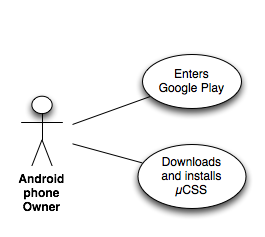
\includegraphics[scale=1]{images/UseCase1}
\end{figure}

    \begin{table}
        \begin{tabular}{|l|l|}
            \hline
            ID               & 1                                                                                                                                  \\ \hline
            Name             & Install $\mu$CSS                                                                                                                   \\
            Goal             & Have $\mu$CSS installed on the Android device                                                                                      \\
            Actors           & Android device owner                                                                                                               \\
            Prequisite       & The actor have a Android device with Google Play                                                                                   \\
            Main Flow        & \begin{itemize} \\ \item{Opens Google Play} \\ \item{Search for ``$\mu$C Software Store''} \\ \item{Installs the application} \\ \end{itemize} \\
            Alternative Flow & None                                                                                                                               \\
            Parent UC        & None                                                                                                                               \\
            Child UC         & All                                                                                                                                \\
            \hline
        \end{tabular}
    \end{table}

\begin{figure}[H]
\centering
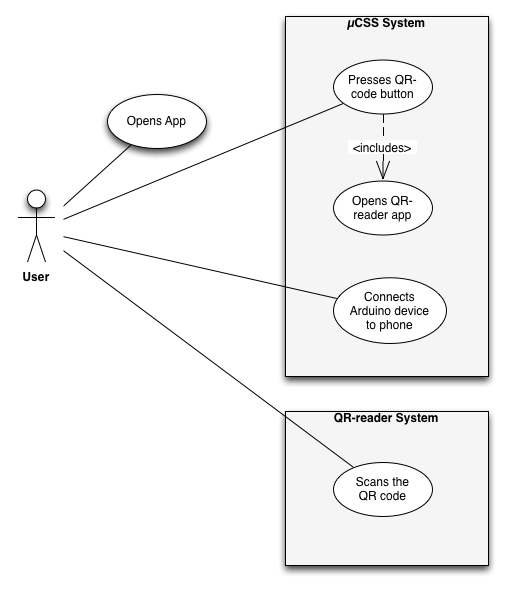
\includegraphics[scale=1]{images/UseCase2}
\end{figure}

\begin{table}
    \begin{tabular}{|l|l|}
        \hline
        ID               & 2                                                                                                                                                                                                                                                                                                          \\ \hline
        Name             & Pair Arduino device and Android device with QR code                                                                                                                                                                                                                                                        \\ 
        Goal             & Connect the Arduino device to the Android application with the use of QR code                                                                                                                                                                                                                              \\ 
        Actors           & Arduino device owner                                                                                                                                                                                                                                                                                       \\ 
        Prerequisite     &     Installed $\mu$CSS \\     Installed predefined QR-reader                                                                                                                                                                                                                                                  \\ 
        End requirement  & The Arduino device is connected to the phone via bluetooth                                                                                                                                                                                                                                                 \\ 
        Main flow        &    \begin{itemize} \\ \item{User opens $\mu$CSS} \\ \item{User presses the button indicating that he wants to pair with the Arduino device using QR code} \\ \item{The system opens the QR reader application} \\ \item{The QR reader application reads the QR code and returns the information it contains} \\ \item{The system pairs with the Arduino device} \\ \end{itemize} \\

 
        Alternative flow & 3.a. The user does not have the right QR code reader installed \\ 3.b. The system prompts the user if he wants to install the QR code reader \\ 3.c. If no: stop \\ 4.a. The QR reader is unable to read the QR code \\ 4.b. Try again or stop                                                             \\ 
        Parent UC        & 1                                                                                                                                                                                                                                                                                                          \\ 
        Child UC         & 7                                                                                                                                                                                                                                                                                                          \\
        \hline
    \end{tabular}
\end{table}

\begin{figure}[H]
\centering
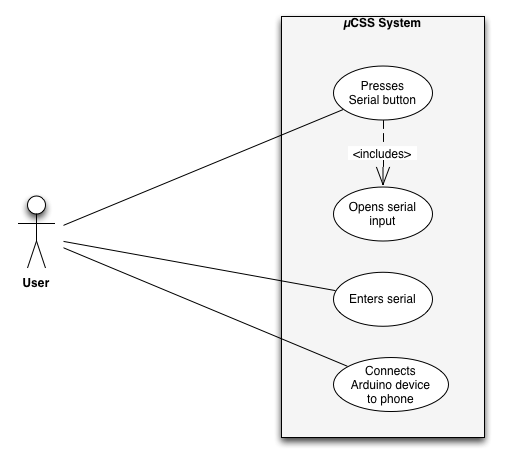
\includegraphics[scale=1]{images/UseCase3}
\end{figure}

\begin{table}
    \begin{tabular}{|l|l|}
        \hline
        ID               & 3                                                                                                                                                                                                                                             \\ \hline
        Name             & Pair Arduino device with Android device using serial                                                                                                                                                                                          \\ 
        Goal             & Connect the Arduino device to the Android application with the use of QR code                                                                                                                                                                 \\ 
        Actors           & Arduino device owner     								             \\ 
        Prerequisite     &     Installed $\mu$CSS \\     Intstalled predefined QR-reader                                                                                                                                                                                 \\ 
        End requirement  & The Arduino device is connected to the phone via bluetooth                                                                                                                                                                                    \\ 
        Main flow        & \begin{itemize} \\ \item{User opens $\mu$CSS} \\ \item{User presses the button indicating that he wants to pair with the Arduino device using a serial code} \\ \item{System opens dialog box for input} \\ \item{The user types the serial} \\ \item{The system pairs with the Arduino device} \\ \end{itemize} \\
 
        Alternative flow & 4.a. The user misspells the serial \\ 4.b. The system displays an error, and prompts again                                                                                                                                                    \\ 
        Parent UC        & 1                                                                                                                                                                                                                                             \\ 
        Child UC         & 7                                                                                                                                                                                                                                             \\
        \hline
    \end{tabular}
\end{table}

\begin{figure}[H]
\centering
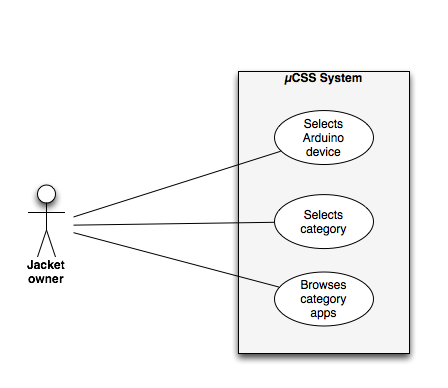
\includegraphics[scale=1]{images/UseCase4}
\end{figure}

        \begin{table}
        \begin{tabular}{|l|l|}
            \hline
            ID               & 4 \\ \hline
            Name             & Browse apps \\
            Actors           & Arduino device owner \\
            Prequisite       & Installed $\mu$CSS \\
            End Requirement  & None \\
            Main Flow        &      
                    \begin{itemize}
                    \item{The user opens $\mu$CSS}
                    \item{The user selects the an Arduino device}
                    \item{The user selects category (One category is named ``al'')}
                    \item{The user browses apps}
                    \end{itemize} \\
            Alternative Flow & 2.a. The user does not select Arduino device, but browses anyway
           \\ \hline
        \end{tabular}
    \end{table}



\begin{figure}[H]
\centering
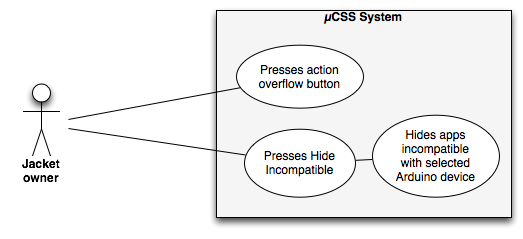
\includegraphics[scale=1]{images/UseCase5}
\end{figure}



\begin{figure}[H]
\centering
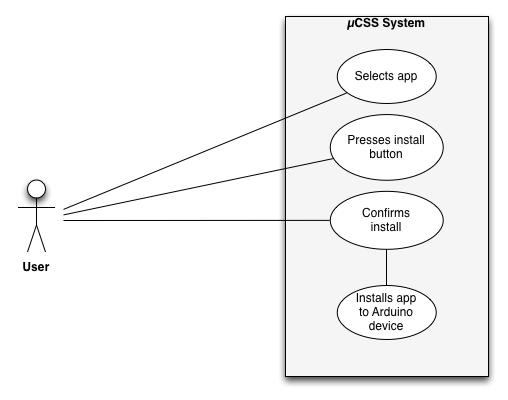
\includegraphics[scale=1]{images/UseCase6}
\end{figure}

\begin{table}
    \begin{tabular}{|l|l|}
        \hline
        ID               & 6                                                                                                                                                                                    \\ \hline
        Name             & Install application on Arduino device                                                                                                                                                \\ 
        Goal             & Connect the Arduino device to the Android application with the use of QR code                                                                                                        \\ 
        Actors           & Arduino device owner                                                                                                                                                                 \\ 
        Prerequisite     &     Installed $\mu$CSS \\     Arduino device connected to $\mu$CSS                                                                                                                   \\ 
        End requirement  & The application is installed on the Arduino device                                                                                                                                   \\ 
        Main flow        &     The user selects the desired application \\     The user presses the “install” button \\     The user confirms the installation \\     The application is installed at the Arduino device \\ 
        Alternative flow & none                                                                                                                                                                                 \\ 
        Parent UC        & 1, 2/3/4, 5                                                                                                                                                                          \\ 
        Child UC         & none                                                                                                                                                                                 \\
        \hline
    \end{tabular}
\end{table}


\section{Mid-term changes}
About halfway through the project we realized that we had to prioritize differently. The over the air transfer of new PUI apps to an arduino device proved to be more demanding than planned. This made us have a talk with the customer about what he wanted us to focus on. \\
\newline
The goal of the project remained consistent with prevoius statement, a simple store application had been made, though not all funcionality was made and tested. Work on this application came to a halt. Resources were now focused primarily on creating an implementation of AVRDude in java without specifically creating it for the application made. The customer wanted to have an implementation of AVRDude in java with intentions of reuse by anyone who might need to through the Apache 2 license. 

\section{Additions}


\section{Deletions}
